\phantomsection\addcontentsline{toc}{section}{\texorpdfstring{第 XV 报告 --- Frobenius 与 $L$ 函数的有理性}{第 XV 报告 --- Frobenius 与 L 函数的有理性}}
\section*{第 XV 报告}
\begin{center}
\Large\bfseries Frobenius 态射与 $L$ 函数的有理性

\medskip
C. Houzel 著
\end{center}

\subsection*{§ 1. Frobenius 态射}

\subsubsection*{第 1 节. Frobenius 自同态}

\begin{statement}{定义 1}
设 $p$ 为素数. 若 $p\cdot 1_{\OO_X}=0$, 则称预概形 $X$ 的特征为 $p$.
\end{statement}

这个条件等价于下述条件: 唯一的态射 $X\to\Spec(\bbZ)$ 可通过 $\Spec(\bF_p)\to\Spec(\bbZ)$ 分解; 而且这样的分解是唯一的.

以 $(\Sch)_p$ 表示预概形范畴中以特征为 $p$ 的预概形为对象的满子范畴. 根据上述说明, 范畴 $(\Sch)_p$ 自然同构于 $\bF_p$-预概形范畴.

若 $X$ 是特征为 $p$ 的预概形, 则对 $\OO_X$ 在任意开集上的每个截面 $f$, 由
\[
\fr_X=(\id_{|X|},\psi),
\qquad \psi:\OO_X\longrightarrow\OO_X,
\qquad \psi(f)=f^p
\]
给出的二元组是 $X$ 的自同态, 因为 $\psi$ 显然是环层 $\OO_X$ 的自同态.

\begin{statement}{定义 2}
设 $X$ 为特征 $p$ 的预概形. 如此定义的自同态 $\fr_X$ 称为 $X$ 的 Frobenius 自同态.
\end{statement}

Frobenius 自同态 $\fr_X$ 函子性地依赖于特征为 $p$ 的预概形 $X$; 即对特征为 $p$ 的预概形之间的每个态射 $g:X\to Y$, 下图交换:
\[
\begin{tikzcd}[column sep=large,row sep=large]
X \arrow[r,"\fr_X"] \arrow[d,"g"'] & X \arrow[d,"g"]\\
Y \arrow[r,"\fr_Y"'] & Y.
\end{tikzcd}
\]
换言之, 我们定义了恒等函子 $\id_{(\Sch)_p}$ 的一个自同态 $\fr$.

\subsubsection*{第 2 节. 相对 Frobenius 态射}

设 $S$ 为特征 $p$ 的预概形; 所有 $S$-预概形的特征也都是 $p$. 若 $X$ 为 $S$-预概形, 则可见 $\fr_X$ 通过投影
\[
\pi_{X/S}:X\times_S(S,\fr_S)\longrightarrow X,
\]
分解, 其中 $(S,\fr_S)$ 表示借助态射 $\fr_S$ 视为 $S$-预概形的 $S$. 以 $X^{(p/S)}$ 表示纤维积 $X\times_S(S,\fr_S)$, 无歧义时也简记为 $X^{(p)}$. 从 $X$ 到 $X^{(p/S)}$ 且与 $\pi_{X/S}$ 复合为 $\fr_X$ 的唯一 $S$-态射记为 $\Fr_{X/S}$; 从而得到如下交换图, 其中的方块为笛卡尔方块.
\[
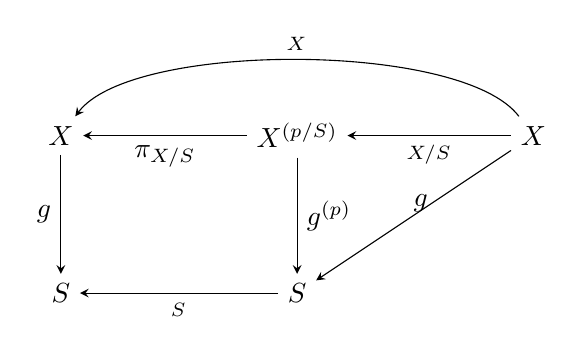
\begin{tikzpicture}[baseline=(current bounding box.center),>=stealth]
\node (XL) at (0,2.0) {$X$};
\node (XM) at (3.0,2.0) {$X^{(p/S)}$};
\node (XR) at (6.0,2.0) {$X$};
\node (SL) at (0,0) {$S$};
\node (SM) at (3.0,0) {$S$};
\draw[->] (XM) -- node[below] {$\pi_{X/S}$} (XL);
\draw[->] (XR) -- node[below] {$\Fr_{X/S}$} (XM);
\draw[->] (XR) .. controls (5.1,3.2) and (0.9,3.2) .. node[above] {$\fr_X$} (XL);
\draw[->] (XL) -- node[left] {$g$} (SL);
\draw[->] (XM) -- node[right] {$g^{(p)}$} (SM);
\draw[->] (XR) -- node[pos=.55,above right] {$g$} (SM);
\draw[->] (SM) -- node[below] {$\fr_S$} (SL);
\end{tikzpicture}
\]

显然, $X^{(p/S)}$ 函子性地依赖于 $S$-预概形 $X$; 函子
\[
p_S:X\longmapsto X^{(p/S)}
\]
就是沿态射 $\fr_S:S\to S$ 的基变换. 与任意基变换一样, 它与投射极限及和交换, 并保持有限型、分离、仿射、射影、平坦、平展等性质. 它与投射极限交换, 因而若 $X$ 带有某种代数结构, 例如群或代数结构, 则 $X^{(p/S)}$ 自然带有同类的代数结构.

利用 $\fr_X$ 关于 $X$ 的函子性, 可见态射 $\Fr_{X/S}$ 函子性地依赖于 $S$-预概形 $X$, 因而定义了函子态射
\[
\Fr_{X/S}:\id_{(\Sch)/S}\longrightarrow p_S
.\]


\begin{statement}{定义 3}
设 $S$ 为特征 $p$ 的预概形, $X$ 为 $S$-预概形. $S$-态射
\[
\Fr_{X/S}:X\longrightarrow X^{(p/S)}
\]
称为 $X$ 相对于 $S$ 的 Frobenius 态射.
\end{statement}

Frobenius 态射的初步形式性质见下述命题.

\begin{statement}{命题 1}
\begin{enumerate}[label=\alph*)]
\item \emph{(传递性.)} 设 $S$ 为特征 $p$ 的预概形, $g:X\to Y$ 为 $S$-预概形之间的 $S$-态射. 联系 $X$, $X^{(p/S)}$, $X^{(p/Y)}$, $Y$, $Y^{(p/S)}$ 和 $S$ 的自然图交换, 且其中三个方块均为笛卡尔方块.
\[
\begin{tikzcd}[column sep=huge,row sep=large]
X \arrow[d,"g"'] & X^{(p/S)} \arrow[l,"\pi_{X/S}"'] \arrow[d,"g^{(p/S)}"] & X^{(p/Y)} \arrow[l] \arrow[d,"g^{(p/Y)}"] & X \arrow[l,"\Fr_{X/Y}"'] \arrow[ll,bend left=35,"\Fr_{X/S}"{description,pos=0.62}] \arrow[dl,"g"] \\
Y \arrow[d] & Y^{(p/S)} \arrow[l,"\pi_{Y/S}"] \arrow[d] & Y \arrow[l,"\Fr_{Y/S}"] \arrow[dl] & {} \\
S & S \arrow[l,"\fr_S"] & {} & {}
\end{tikzcd}
\]

\item \emph{(基变换.)} 设 $g:S'\to S$ 为特征 $p$ 的预概形之间的态射, $X$ 为 $S$-预概形. 存在关于 $X$ 函子性的典范同构
\[
X^{(p/S)}\times_S S'\simeq (X\times_S S')^{(p/S')}
\]
即以撇号表示沿 $g$ 基变换的结果时, 有 $(X^{(p/S)})'\simeq X'{}^{(p/S')}$. 此外, 通过上述同构作等同后, 有
\[
\Fr_{X'/S'}=(\Fr_{X/S})'
.\]

\end{enumerate}
\end{statement}

证明是直接的.

\begin{statement}{命题 2}
设 $S$ 为特征 $p$ 的预概形, $X$ 为 $S$-预概形.
\begin{enumerate}[label=\alph*)]
\item 相对 Frobenius 态射
\[
\Fr_{X/S}:X\longrightarrow X^{(p/S)}
\]
是整的、满的且根的; 因而它是泛同胚.

\item 若 $X\to S$ 为开浸入, 则 $X^{(p)}=X$ 且 $\Fr_{X/S}=\id_X$. 若 $X\to S$ 为闭浸入, 将 $X$ 等同于 $S$ 的闭赋环子空间 $(|X|,\OO_S/\JJ)$, 则
\[
X^{(p)}=(|X|,\OO_S/\JJ^p)
\]
\sgacollationmark{XV-04}且 $\Fr_{X/S}=(\id_{|X|},\varphi)$, 其中 $\varphi:\OO_S/\JJ^p\to\OO_S/\JJ$ 为显然的增广映射.

\item 设 $X$ 在 $S$ 上局部有限表示.
\begin{enumerate}[label=\arabic*)]
\item 下列三个条件等价:
\[
\begin{array}{ll}
\text{(i)}& X\text{ 在 }S\text{ 上非分歧},\\
\text{(ii)}& \Fr_{X/S}\text{ 非分歧},\\
\text{(iii)}& \Fr_{X/S}\text{ 是单态射}.
\end{array}
\]
\item 类似地, 下列三个条件等价:
\[
\begin{array}{ll}
\text{(i')}& X\text{ 在 }S\text{ 上平展},\\
\text{(ii')}& \Fr_{X/S}\text{ 平展},\\
\text{(iii')}& \Fr_{X/S}\text{ 是同构}.
\end{array}
\]
\end{enumerate}
\end{enumerate}
\end{statement}

先证 a). 复合 $\pi_{X/S}\circ\Fr_{X/S}=\fr_X$ 显然是整的、满的且根的; 因而 $\Fr_{X/S}$ 是根态射 (EGA I 3.5.6 (ii)). 此外, $\pi_{X/S}$ 是由 $\fr_S$ 沿 $X\to S$ 基变换而得的, 因此它分离且为根态射; 于是 $\Fr_{X/S}$ 是整态射 (EGA II 6.1.5 (v)) 且为满态射.

b) 的证明显然, 只需注意对 $\OO_S$ 的每个理想 $\JJ$ 都有
\[
\JJ\OO_{(S,\fr_S)}=\JJ^p
.\]


c) 的证明. 已知一个态射为单态射 (分别为同构) 的充要条件是它为根态射且非分歧 (分别为根态射、平展且满). 这就给出了 (ii) 与 (iii) 以及 (ii\textquotesingle) 与 (iii\textquotesingle) 的等价性. 余下需证 (i) 与 (ii) 等价, 以及 (i\textquotesingle) 与 (ii\textquotesingle) 等价.

为此, 使用非分歧性的微分判据 (SGA I 3), 以及同构
\[
\Omega^1_{X/S}\simeq \Omega^1_{X/X^{(p)}}
\]
这个同构由典范正合列
\[
\Fr_{X/S}^*(\Omega^1_{X^{(p)}/S})\longrightarrow \Omega^1_{X/S}
\longrightarrow \Omega^1_{X/X^{(p)}}\longrightarrow 0
\]
(SGA II 4) 给出. 该正合列的第一个箭头显然为零, 因为 $\Omega^1_{X^{(p)}/S}$ 由 $\OO_{X^{(p)}}$ 的截面的微分生成, 而微分 $d_{X/S}$ 在 $(\OO_X)^p$ 和 $\OO_S$ 上均为零. 因而 (i) 与 (ii) 等价.

现设 $X$ 在 $S$ 上平展; 由基变换, $X^{(p)}$ 也如此, 因而态射 $\Fr_{X/S}:X\to X^{(p)}$ 平展. 反之, 设 $\Fr_{X/S}$ 平展; 它非分歧, 从而 $X$ 在 $S$ 上非分歧. 换言之, 结构态射 $g:X\to S$ 在 $X$ 上对平展拓扑局部地为闭浸入 (SGA I, 推论 7.8). 因此可设 $g$ 为有限表示的闭浸入, 只需证明若 $\Fr_{X/S}$ 是同构, 则 $g$ 是开浸入. 现在 $X$ 由有限型理想 $\JJ$ 定义,
\[
X=(|X|,\OO_S/\JJ),
\]
而由 b),
\[
X^{(p)}=(|X|,\OO_S/\JJ^p),
\qquad
\Fr_{X/S}=(\id_{|X|},\OO_S/\JJ^p\to\OO_S/\JJ).
\]
故 $\Fr_{X/S}$ 为同构等价于 $\JJ=\JJ^p$; 由于 $\JJ$ 为有限型, Nakayama 引理说明对每一点 $s\in S$, 或有 $\JJ_s=0$, 或有 $\JJ_s=\OO_{S,s}$, 从而得到结论.

\subsubsection*{第 3 节. 对模的作用. 例}

设 $S$ 为特征 $p$ 的预概形, $X$ 为 $S$-预概形. 对每个作为 Zariski 拓扑上的层的 $\OO_X$-模 $\cE$, 置
\[
\cE^{(p/S)}=\pi_{X/S}^*(\cE)=\cE\otimes_{\OO_X}\OO_{X^{(p)}}
 =\cE\otimes_{\OO_S}\OO_{(S,\fr_S)}.
\]
这是一个 $\OO_{X^{(p)}}$-模, 且有
\[
\cE^{(p/X)}\simeq \Fr_{X/S}^*(\cE^{(p/S)}).
\]

最值得注意的是 $X=S$ 的情形; 此时可以无歧义地以 $\cE^{(p)}$ 代替 $\cE^{(p/S)}$, 并且 $\cE^{(p)}=\fr_S^*(\cE)$. 伴随态射
\[
\cE\longrightarrow \fr_{S*}\fr_S^*(\cE)
\]
是阿贝尔层的态射 $\cE\to\cE^{(p)}$, 它并非 $\OO_S$-线性的, 而是通常意义下的 ``$p$-线性'' 态射; 显然, 它是从 $\cE$ 到一个 $\OO_S$-模的泛 $p$-线性态射.

显然, $\cE^{(p)}$ 函子性地依赖于 $\cE$, 且函子 $\cE\mapsto\cE^{(p)}$ 右正合, 但一般不正合; 它与张量积交换:
\[
(\cE\otimes_{\OO_X}\cF)^{(p)}\simeq
\cE^{(p)}\otimes_{\OO_{X^{(p)}}}\cF^{(p)},
\]
并且保持拟凝聚、有限型、有限表示、平坦、局部自由等性质. 特别地, 若 $\cL$ 为 $S$ 上的可逆层, 则立即可见 $\cL^{(p)}$ 典范同构于 $\cL^{\otimes p}$, 因为将截面取第 $p$ 次张量幂所定义的态射 $\cL\to\cL^{\otimes p}$ 是泛 $p$-线性态射.

若 $\mathcal{A}$ 为 $\OO_S$-代数, 则 $\mathcal{A}^{(p)}$ 带有从 $\mathcal{A}$ 的代数结构导出的 $\OO_S$-代数结构. 设 $\mathcal{A}$ 拟凝聚 (分别为分次且拟凝聚), 则 $\mathcal{A}^{(p)}$ 也如此, 而且有
\[
\Spec(\mathcal{A}^{(p)})=\Spec(\mathcal{A}\otimes_{\OO_S}\OO_{(S,\fr_S)})
 \simeq \Spec(\mathcal{A})\times_S(S,\fr_S)=\Spec(\mathcal{A})^{(p)},
\]
分别有
\[
\Proj(\mathcal{A}^{(p)})=\Proj(\mathcal{A}\otimes_{\OO_S}\OO_{(S,\fr_S)})
 \simeq \Proj(\mathcal{A})\times_S(S,\fr_S)=\Proj(\mathcal{A})^{(p)}.
\]
投影 $\pi_{\Spec(\mathcal{A})/S}:\Spec(\mathcal{A})^{(p)}\to\Spec(\mathcal{A})$ (分别为 $\pi_{\Proj(\mathcal{A})/S}$) 等同于由 $\mathcal{A}\to\mathcal{A}^{(p)}$ 导出的态射. 另一方面, $\Fr_{\Spec(\mathcal{A})/S}$ (分别为 $\Fr_{\Proj(\mathcal{A})/S}$) 来自一个 $\OO_S$-代数同态
\[
\mathcal{A}^{(p)}=\mathcal{A}\otimes_{\OO_S}\OO_{(S,\fr_S)}\longrightarrow \mathcal{A}
\]
对 $\mathcal{A}$ 的每个截面 $a$ 和 $\OO_S$ 的每个截面 $f$, 它将 $a\otimes f$ 映为 $a^p f$. 为说明这一点, 只需注意将 $\mathcal{A}\to\mathcal{A}^{(p)}$ 先作用、再作用此同态所得的复合, 就是在 $\mathcal{A}$ 中取第 $p$ 次幂.

考虑 $\mathcal{A}$ 是拟凝聚 $\OO_S$-模 $\cE$ 的对称代数 $\Sym(\cE)$ 的特殊情形; 显然 $\mathcal{A}^{(p)}\simeq\Sym(\cE^{(p)})$, 因而
\[
\mathbb V(\cE^{(p)})\simeq\Spec(\mathcal{A}^{(p)})\simeq\Spec(\mathcal{A})^{(p)}=\mathbb V(\cE)^{(p)},
\]
\[
\mathbb P(\cE^{(p)})\simeq\Proj(\mathcal{A}^{(p)})\simeq\Proj(\mathcal{A})^{(p)}=\mathbb P(\cE)^{(p)}.
\]
至于 $\Fr_{\mathbb V(\cE)/S}$ (分别为 $\Fr_{\mathbb P(\cE)/S}$), 则有如下分解:
\[
\mathbb V(\cE)\longrightarrow \mathbb V(\Sym^p(\cE))\longrightarrow \mathbb V(\cE^{(p)}),
\]
分别有
\[
\mathbb P(\cE)\longrightarrow \mathbb P(\Sym^p(\cE))\longrightarrow \mathbb P(\cE^{(p)}),
\]
其中第一个箭头由典范态射
\[
\Sym(\Sym^p(\cE))\longrightarrow \Sym(\cE)
\]
定义, 后者来自 $\Sym^p(\cE)\to\Sym(\cE)$; 第二个箭头则由 $\OO_S$-模态射
\[
\cE^{(p)}\longrightarrow \Sym^p(\cE)
\]
定义, 后者来自将截面取第 $p$ 次对称幂所给出的 $p$-线性态射 $\cE\to\Sym^p(\cE)$. 在 $X=\mathbb P(\cE)$ 的情形, 计算其基本层 $\OO_{X^{(p)}}(1)$, 得
\[
\OO_{X^{(p)}}(1)=(\Sym(\cE)^{(p)}(1))^{\sim}
=(\Sym(\cE)(1)^{(p)})^{\sim}
\simeq \OO_X(1)^{(p/S)}.
\]
当 $\cE=\OO_S^n$, $\Sym(\cE)=\OO_S[T_1,\ldots,T_n]$ 且 $X=\mathbb V(\cE)=S[T_1,\ldots,T_n]$ (分别为 $X=\mathbb P(\cE)=\mathbb P_S^{n-1}$) 时, 显然 $\cE^{(p)}\simeq\OO_S^n=\cE$, 从而 $X^{(p)}=X$. Frobenius 态射 $\Fr_{X/S}$ 来自代数 $\OO_S[T_1,\ldots,T_n]$ 中将 $T_i$ 映为 $T_i^p$ $(i=1,\ldots,n)$ 的自同态.

现考虑在 $S$ 上仿射且有限型 (分别为射影) 的预概形 $X$, 它由理想 (分别为齐次理想)
\[
\JJ\subset \OO_S[T_1,\ldots,T_n].
\]
定义. 于是 $X=\Spec(\mathcal{A})$ (分别为 $X=\Proj(\mathcal{A})$), 其中
\[
\mathcal{A}=\OO_S[T_1,\ldots,T_n]/\JJ.
\]
可见
\[
\mathcal{A}^{(p)}
\simeq \OO_S[T_1,\ldots,T_n]/\JJ',
\]
其中 $\JJ'$ 为
$\JJ^{(p)}=\JJ\otimes_{\OO_S}\OO_{(S,\fr_S)}$ 在 $\OO_S[T_1,\ldots,T_n]$ 中的像; 理想 $\JJ'$
是将 $\JJ$ 中多项式的系数取第 $p$ 次幂得到的.
有 $X^{(p)}=\Spec(\mathcal{A}^{(p)})$ (分别为 $\Proj(\mathcal{A}^{(p)})$), 且 Frobenius 态射
\[
\Fr_{X/S}:X\longrightarrow X^{(p)}
\]
由将坐标 $T_i$ 取第 $p$ 次幂定义; 这就确定了态射 $\mathcal{A}^{(p)}\to\mathcal{A}$.


\subsection*{4. 迭代 Frobenius 态射; 完美预概形}

对每个整数 $\nu\geq0$, 迭代自同态 $\fr_X^\nu$ 函子性地依赖于特征为 $p$ 的预概形 $X$. 因此, 若 $S$ 为特征 $p$ 的预概形, $X$ 为 $S$-预概形, 则 $\fr_X^\nu$ 唯一分解为 $S$-态射
\[
\Fr_{X/S}^\nu:X\longrightarrow X^{(p^\nu/S)},
\]
(其中
\[
X^{(p^\nu/S)}=X\times_S(S,\fr_S^\nu),
\]
) 与投影 $X^{(p^\nu/S)}\to X$ 的复合. 态射 $\Fr_{X/S}^\nu$ 函子性地依赖于 $S$-预概形 $X$, 并与基底 $S$ 的变换相容 (参见第 2 节命题 1b)). 此外显然有
\[
X^{(p^\nu/S)}=X^{(p^\nu)}\simeq\bigl(X^{(p^{\nu-1})}\bigr)^{(p)}
\]
及
\[
\Fr_{X/S}^\nu=(\Fr_{X/S}^{\nu-1})^{(p)}\circ\Fr_{X/S},
\]
这里通过上述典范同构作了等同.

\begin{statement}{定义 4}
若 $\fr_S$ 为 $S$ 的自同构, 则称特征为 $p$ 的预概形 $S$ 为完美的.
\end{statement}

若 $S$ 为特征 $p$ 的完美预概形, $X$ 为 $S$-预概形, 则立即可见 $X^{(p/S)}$ 可等同于借助态射 $\fr_S^{-1}\circ g:X\to S$ 视为 $S$-预概形的预概形 $X$, 其中 $g$ 为 $X$ 到 $S$ 的结构态射; 在这一等同下, $\Fr_{X/S}=\fr_X$.

作为完美预概形的一个例子, 下文将用到 $S=\Spec(\mathbb F_q)$, 其中 $q=p^\nu$ 为特征 $p$ 的幂; 事实上, 此时 $\fr_S^\nu=\id_S$. 若 $X$ 为 $S$-预概形, 则可见
\[
X^{(p^\nu/S)}=X,
\qquad
\Fr_{X/S}^\nu=\fr_X^\nu.
\]
注意 $\nu=1$ 时得到 $S=\Spec(\mathbb F_p)$, 此时 $\fr_S=\id_S$; $S$-预概形就是特征为 $p$ 的预概形; 在这个基底 $S$ 上, 有 $X^{(p/S)}=X$ 且 $\Fr_{X/S}=\fr_X$.

\section*{§ 2. Frobenius 对应}

\subsection*{1. 定义}

设 $X$ 为特征 $p$ 的预概形, $F$ 为 $X_{\et}$ 上的集合层. 对每个平展 $X$-预概形 $U$, 有
\[
(\fr_X)_*(F)(U)=F(\fr_X^{-1}(U))=F(U^{(p/X)}),
\]
而 Frobenius 态射 $\Fr_{U/X}:U\to U^{(p/X)}$ 定义了映射
\[
F(\Fr_{U/X}):\fr_{X*}(F)(U)\longrightarrow F(U),
\]
此映射显然关于 $U$ 函子化 (因为 $\Fr_{U/X}$ 关于 $U$ 函子化). 因而得到 $X_{\et}$ 上的层态射:
\[
(\fr_X)_*(F)\longrightarrow F.
\]
当 $U$ 在 $X$ 上平展时, $\Fr_{U/X}$ 是同构 (§ 1 第 2 节命题 2c)), 因而 $F(\Fr_{U/X})$ 也是同构; 所以上述态射是同构. 当 $F$ 带有代数结构时, 例如当它为 $\Lambda$-模层而 $\Lambda$ 为给定的基环时, 这个同构与代数结构相容. 由于 $(\fr_X)^*$ 为函子 $(\fr_X)_*$ 的左伴随, 这个同构的逆
\[
F(\Fr_{/X})^{-1}:F\longrightarrow \fr_{X*}(F)
\]
定义了态射
\[
\Fr^*_{F/X}:(\fr_X)^*(F)\longrightarrow F.
\]
还可以进一步断言: 由于 $\fr_X$ 为泛同胚 (§ 1 第 2 节命题 2a)), 函子 $(\fr_X)^*$ 与 $(\fr_X)_*$ 互为拟逆; 因而 $\Fr^*_{F/X}$ 是同构, 如同导出它的态射 $F(\Fr_{/X})^{-1}$ 一样.

\begin{statement}{定义 1}
给定特征为 $p$ 的预概形 $X$ 和 $X_{\et}$ 上的集合层 $F$, $(X,F)$ 上的 Frobenius 对应是由 $X$ 的 Frobenius 自同态 $\fr_X$ 与同构
\[
\Fr^*_{F/X}=(F(\Fr_{/X})^{-1})^\sharp:(\fr_X)^*(F)\longrightarrow F.
\]组成的二元组 $(\fr_X,\Fr^*_{F/X})$.
\end{statement}

当然, 对每个整数 $\nu\geq0$, 可以同样定义迭代 Frobenius 对应 $(\fr_X^\nu,(\Fr^*_{F/X})^\nu)$; 当 $\nu\geq1$ 时, 同构
\[
(\Fr^*_{F/X})^\nu:(\fr_X^\nu)^*(F)\longrightarrow F
\]
等于
\[
(\Fr^*_{F/X})^{\nu-1}\circ (\fr_X^{\nu-1})^*(\Fr^*_{F/X})
\]
也等于
\[
\Fr^*_{F/X}\circ\fr_X^*((\Fr^*_{F/X})^{\nu-1})
.\]


考察特殊情形: $F$ 由 $X$ 上的平展预概形 $V$ 表示. 此时 $(\fr_X)^*(F)=V^{(p/X)}$, $F(V)=\Hom_X(V,V)$,
\[
(\fr_X)^*(F)(V)=F(V^{(p/X)})=\Hom_X(V^{(p/X)},V),
\]
且 $F(\Fr_{V/X})$ 为从 $\Hom_X(V^{(p/X)},V)$ 到 $\Hom_X(V,V)$ 的映射, 将态射 $\psi$ 映为 $\psi\circ\Fr_{V/X}$. 于是 $\Fr^*_{F/X}$ 等同于从 $V^{(p/X)}$ 到 $V$ 的态射, 它是 $\id_V$ 在上述映射的逆映射 $F(\Fr_{V/X})^{-1}$ 下的像. 这表明, 当 $F=V$ 在 $X$ 上平展时, 有
\[
\Fr^*_{V/X}=(\Fr_{V/X})^{-1}.
\]

注意, 若层 $F$ 为常值层, 则显然有
\[
(\fr_X)^*(F)=F,
\qquad
\Fr^*_{F/X}=\id_F.
\]

\begin{statement}{命题 1}
\begin{enumerate}[label=\alph*)]
\item 同构 $\Fr^*_{F/X}$ 函子性地依赖于层 $F$; 换言之, 有函子同构
\[
\Fr^*_{/X}:\fr_X^*\longrightarrow \id_{\widetilde X_{\et}},
\]
其中 $\widetilde X_{\et}$ 为 $X_{\et}$ 上的集合层范畴.
\item $(X,F)$ 上的 Frobenius 对应 $(\fr_X,\Fr^*_{F/X})$ 与基底 $X$ 的变换相容. 即若以 $\mathcal F$ 表示 $(\Sch)_p$ 上的纤维范畴, 其对象为可变的特征 $p$ 预概形上的平展层, 则函子 $\fr_X^*$, $X\in\Ob(\Sch)_p$, 定义了笛卡尔 $(\Sch)_p$-函子
\[
\fr^*: \mathcal F\longrightarrow\mathcal F,
\]
而态射 $\Fr^*_{F/X}$, $X\in\Ob(\Sch)_p$, $F\in\Ob\widetilde X_{\et}$, 定义了函子性的 $(\Sch)_p$-态射
\[
\Fr^*_{/}:\fr^*\longrightarrow\id_{\mathcal F}
\]
且它是同构.
\item 反过来, 这些性质刻画了 $\Fr^*_{/}$; 即从 $\fr^*$ 到 $\id_{\mathcal F}$ 恰有一个函子性的 $(\Sch)_p$-态射.
\end{enumerate}
\end{statement}

注意 b) 的陈述蕴含 a) 的陈述; 后者完全是显然的.

证明 b). 设 $g:X'\to X$ 为特征 $p$ 的预概形之间的态射, $F$ 为 $X_{\et}$ 上的层. 置 $F'=g^*(F)$, 更一般地, 对 $X$ 上给定的任意对象, 用撇号标记它沿 $g$ 的逆像. 由于
\[
g\circ\fr_{X'}=\fr_X\circ g,
\]
有
\[
\fr_{X'}^*(F')=\fr_{X'}^*(g^*F)=g^*(\fr_X^*F)=(\fr_X^*F)',
\]
因而这些 $\fr_X^*$ 定义了 $(\Sch)_p$ 上的笛卡尔函子 $\fr^*$. 余下需证
\[
\Fr^*_{F'/X'}=(\Fr^*_{F/X})'.
\]
利用伴随函子的性质, 可见这等价于证明: $F'(\Fr_{/X'})^{-1}$ 在双射
\[
\Hom_{X'}(F',\fr_{X'*}(F'))
 =\Hom_{X'}(g^*F,\fr_{X'*}g^*F)
 \simeq \Hom_X(F,g_*\fr_{X'*}g^*F)
\]
(其中 $g^*$ 为 $g_*$ 的左伴随) 下的像, 等于 $F(\Fr_{/X})^{-1}$ 在由伴随态射 $F\xrightarrow{\alpha}g_*g^*F$ 所定义的映射
\[
\Hom_X(F,\fr_{X*}F)\longrightarrow
\Hom_X(F,\fr_{X*}g_*g^*F)=
\Hom_X(F,g_*\fr_{X'*}g^*F)
\]
下的像; 换言之, 需证
\[
\alpha\circ F(\Fr_{/X})=g_*(F'(\Fr_{/X'}))\circ\fr_{X*}(\alpha),
\]
这就是说, 对每个在 $X$ 上平展的预概形 $U$, 下图交换:
\[
\begin{tikzcd}[column sep=large,row sep=large]
F(U^{(p/X)}) \arrow[r,"F(\Fr_{U/X})"] \arrow[d]
& F(U) \arrow[d]\\
F'(U'{}^{(p/X')}) \arrow[r,"F'(\Fr_{U'/X'})"']
& F'(U') ,
\end{tikzcd}
\]
其中竖直箭头为典范映射. 但这立即由
\[
\Fr_{U'/X'}=(\Fr_{U/X})'
\]
(§ 1 第 2 节命题 1b)) 得出.

为证 c), 与 $(\Fr^*_{/})^{-1}$ 复合后, 只需证明 $\id_{\mathcal F}$ 仅有一个 $(\Sch)_p$-自同态, 即恒等态射. 设 $\psi$ 为 $\id_{\mathcal F}$ 的 $(\Sch)_p$-自同态, $F$ 为特征 $p$ 的预概形 $X$ 上的层, $U$ 为 $X$ 上的平展预概形. 已知 $F(U)$ 等同于 $\Hom_U(U,F|U)$, 而 $\psi_F(U):F(U)\to F(U)$ 等同于映射
\[
s\longmapsto \psi_{F|U}\circ s=s\circ\psi_U,
\]
其中 $s\in\Hom_U(U,F|U)$. 由于 $\widetilde U_{\et}$ 的终层 $U$ 除恒等态射外没有其他自同态, 故 $\psi_U=\id_U$. 因而 $\psi_F(U)$ 也是 $F(U)$ 的恒等态射, 从而 $\psi=\id_{\mathcal F}$.

当然, 若层 $F$ 带有代数结构, 则同构 $\Fr^*_{F/X}$ 与此结构相容; 例如, 若 $F$ 为特征 $p$ 的预概形 $X$ 上的群层, 则 $\Fr^*_{F/X}$ 为群层的同构. 设 $\Lambda$ 为环, $F$ 为 $X$ 上的 $\Lambda$-模层; 则 $\Fr^*_{F/X}$ 为 $\Lambda$-模层的同构. 更一般地, 若 $F^\bullet$ 为 $\Lambda$-模复形, 则可立即定义同构
\[
\Fr^*_{F^\bullet/X}:\fr_X^*(F^\bullet)\longrightarrow F^\bullet
\]
根据命题 1a), 它在次数 $i$ 的分量上等于 $\Fr^*_{F^i/X}$. 此时, 二元组 $(\fr_X,\Fr^*_{F^\bullet/X})$ 确实是通常意义下 $(X,F^\bullet)$ 上的对应; 这个对应关于 $F^\bullet$ 函子化, 并与基底 $X$ 的变换相容 (命题 1a), b)).

\subsection*{2. 对上同调的作用}

\begin{statement}{命题 2}
设 $X$ 为特征 $p$ 的预概形.
\begin{enumerate}[label=\alph*)]
\item 对 $X_{\et}$ 上的每个集合层 $F$, 由 $(\fr_X,\Fr^*_{F/X})$ 定义的 $H^0(X,F)$ 的自同态, 即复合
\[
H^0(X,F)\longrightarrow H^0(X,\fr_X^*(F))\longrightarrow H^0(X,F),
\]
为 $H^0(X,F)$ 的恒等态射. 其中第一个箭头是由 $H^0(X,F)$ 关于 $X$ 的反变性导出的典范映射, 第二个箭头为 $H^0(X,\Fr^*_{F/X})$.
\item 对 $X_{\et}$ 上的每个群层 $F$, 由 $(\fr_X,\Fr^*_{F/X})$ 定义的 $H^1(X,F)$ 的自同态, 即
\[
H^1(X,F)\longrightarrow H^1(X,\fr_X^*F)\longrightarrow H^1(X,F),
\]
为恒等态射.
\item 对 $X_{\et}$ 上的每个左有界 $\Lambda$-模复形 $F$, 由 $(\fr_X,\Fr^*_{F/X})$ 定义的 $\RGamma_X(F)$ 的自同态, 即复合
\[
\RGamma_X(F)\longrightarrow \RGamma_X(\fr_X^*F)\longrightarrow \RGamma_X(F),
\]
为恒等态射.
\end{enumerate}
\end{statement}

先证明 a), 再由它推出 b) 和 c). 以 $\psi_F$ 表示所考察的 $H^0(X,F)$ 的自同态. 显然 $\psi_F$ 函子性地依赖于 $F$, 且 $\psi_X=\id_{H^0(X,X)}$. $H^0(X,F)$ 的每个元素 $s$ 等同于层态射 $s:X\to F$, 并且 $s$ 是 $H^0(X,X)$ 中唯一元素在 $H^0(X,s)$ 下的像; 根据上述说明, 由于
\[
\psi_F\circ H^0(X,s)=H^0(X,s)\circ\psi_X=H^0(X,s),
\]
可见对每个 $s$ 都有 $\psi_F(s)=s$, 从而 $\psi_F=\id_{H^0(X,F)}$.

注意 $\psi_F$ 也等于复合
\[
H^0(X,F)\longrightarrow H^0(X,\fr_{X*}F)
\longrightarrow H^0(X,F),
\]
其中第一个箭头为 $H^0(X,F(\Fr_{/X})^{-1})$, 第二个箭头为典范映射, 也就是恒等映射. 类似地, b) 和 c) 中所考察的自同态分别分解为
\[
H^1(X,F)\longrightarrow H^1(X,\fr_{X*}F)
\longrightarrow H^1(X,F),
\]
以及
\[
\RGamma_X(F)\longrightarrow \RGamma_X(\fr_{X*}F)
\longrightarrow \RGamma_X(F).
\]

为证明 b), 取一个将 $F$ 嵌入某个群层 $G$ 的单态射 $F\to G$, 使得 $H^1(X,G)=0$. 则 $\fr_{X*}F\to\fr_{X*}G$ 为单态射, 且 $H^1(X,\fr_{X*}G)=0$. 引入商齐性集合层 $C=G/F$. 由于 $\fr_X$ 整、满且为根态射, 函子 $\fr_X^*$ 和 $\fr_{X*}$ 是互为拟逆的范畴等价 (SGA VIII 定理 1.1). 因此
\[
\fr_{X*}(C)\simeq\fr_{X*}(G)/\fr_{X*}(F),
\]
而上同调正合列 (SGA XII 命题 3.1) 表明, 所考察的 $H^1(X,F)$ 的自同态是由
\[
\psi_C:H^0(X,C)\longrightarrow H^0(X,C),
\]
通过取商而来; 由 a), 后者为恒等态射. 因而所考察的自同态为 $\id_{H^1(X,F)}$.

c) 的证明类似: 使用由 $\Lambda$-模构成的复形 $I$, 使其在每个次数上内射, 且在导出范畴 $D^+$ 中同构于 $F$. 由于 $\fr_{X*}$ 为范畴等价, 复形 $\fr_{X*}(I)$ 在每个次数上内射, 且在 $D^+$ 中同构于 $\fr_{X*}(F)$. 于是可将 $\RGamma_X(F)$ 等同于 $H^0(X,I)$, 将 $\RGamma_X(\fr_{X*}F)$ 等同于 $H^0(X,\fr_{X*}I)$; 可见所考察的 $\RGamma_X(F)$ 的自同态等同于 $\psi_I$, 而后者为恒等态射. 因而所考察的自同态为 $\id_{\RGamma_X(F)}$.

\subsection*{3. 积的性质}

设 $X$ 和 $X'$ 为特征 $p$ 的预概形. 它们的积 $X\times X'$ 就是纤维积 $X\times_eX'$, 其中 $e=\Spec(\mathbb F_p)$. 显然
\[
\fr_{X\times X'}=\fr_X\times\fr_{X'}=(\fr_X\times\id_{X'})\circ(\id_X\times\fr_{X'})
=(\id_X\times\fr_{X'})\circ(\fr_X\times\id_{X'}).
\]
立即推出, 对每个 $X$-预概形 $Y$ 和每个 $X'$-预概形 $Y'$, 存在典范同构
\[
(Y\times Y')^{(p/X\times X')}
\simeq Y^{(p/X)}\times Y'{}^{(p/X')};
\]
在此同构下, 可以写成
\[
\Fr_{Y\times Y'/X\times X'}=\Fr_{Y/X}\times\Fr_{Y'/X'}.
\]

\begin{statement}{命题 3}
设 $X$ 和 $X'$ 为特征 $p$ 的预概形, $\Lambda$ 为交换环, $F$ 为 $X_{\et}$ 上的 $\Lambda$-模层, $F'$ 为 $X'_{\et}$ 上的 $\Lambda$-模层. 有
\[
\begin{aligned}
\Fr^*_{F\boxt_\Lambda F'/X\times X'}
&=\Fr^*_{F/X}\otimes\Fr^*_{F'/X'}\\
&=(\id_F\otimes\Fr^*_{F'/X'})
  \circ(\Fr^*_{F/X}\otimes\id_{\fr_{X'}^*F'})\\
&=(\Fr^*_{F/X}\otimes\id_{F'})
  \circ(\id_{\fr_X^*F}\otimes\Fr^*_{F'/X'}).
\end{aligned}
\]
\end{statement}

在写出这些等式时, 已通过典范同构将
\[
\fr_{X\times X'}^*(F\boxt_\Lambda F')
\]
等同于张量积 $\fr_X^*(F)\otimes_\Lambda\fr_{X'}^*(F')$.

第一个等式的两边关于 $F$ 和 $F'$ 函子化, 并与基底 $X$ 或 $X'$ 的变换相容. 而且它们与关于 $F$ 或 $F'$ 取归纳极限相容, 因为张量积与归纳极限交换, 且显然
\[
\Fr^*_{(\varinjlim F_i)/X}=\varinjlim\Fr^*_{F_i/X};
\]
因而可归结为 $F=\Lambda_X$ 和 $F'=\Lambda_{X'}$ 的情形, 此时结论显然.

\begin{statement}{推论}
在命题 3 的条件下, 分别由
\[
(\id_X\times\fr_{X'},\,\id_F\otimes\Fr^*_{F'/X'})
\]
及
\[
(\fr_X\times\id_{X'},\,\Fr^*_{F/X}\otimes\id_{F'})
\]
定义的 $\RGamma_{X\times X'}(F\boxt F')$ 的自同态是互逆的同构.
\end{statement}

以 $\psi'$ 和 $\psi$ 表示这些自同态, 例如证明 $\psi\circ\psi'=\id$. 这由下述交换图得出:
\[
\resizebox{\textwidth}{!}{%
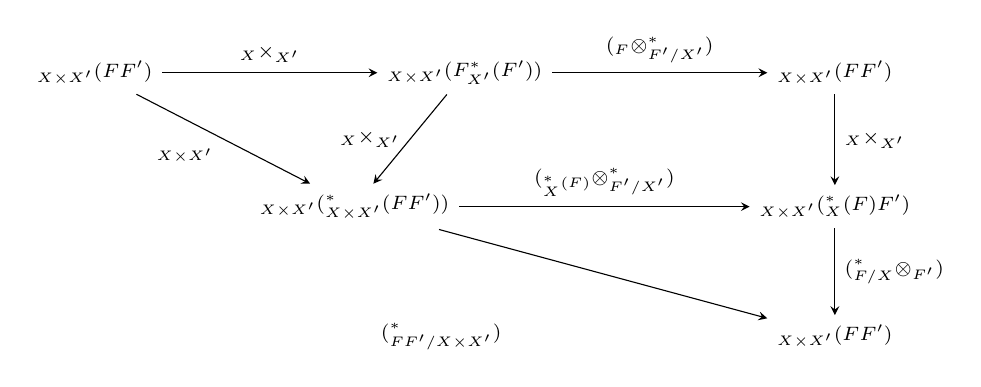
\begin{tikzpicture}[baseline=(current bounding box.center),>=stealth,font=\scriptsize]
\node (A) at (0,3.6) {$\RGamma_{X\times X'}(F\boxt F')$};
\node (B) at (4.7,3.6) {$\RGamma_{X\times X'}(F\boxt\fr_{X'}^*(F'))$};
\node (C) at (9.4,3.6) {$\RGamma_{X\times X'}(F\boxt F')$};
\node (D) at (3.3,1.9) {$\RGamma_{X\times X'}(\fr^*_{X\times X'}(F\boxt F'))$};
\node (E) at (9.4,1.9) {$\RGamma_{X\times X'}(\fr_X^*(F)\boxt F')$};
\node (F) at (4.4,0.25) {$\RGamma(\Fr^*_{F\boxt F'/X\times X'})$};
\node (G) at (9.4,0.25) {$\RGamma_{X\times X'}(F\boxt F')$};
\draw[->] (A) -- node[above] {$\id_X\times\fr_{X'}$} (B);
\draw[->] (B) -- node[above] {$\RGamma(\id_F\otimes\Fr^*_{F'/X'})$} (C);
\draw[->] (A) -- node[below left] {$\fr_{X\times X'}$} (D);
\draw[->] (B) -- node[left] {$\fr_X\times\id_{X'}$} (D);
\draw[->] (C) -- node[right] {$\fr_X\times\id_{X'}$} (E);
\draw[->] (D) -- node[above] {$\RGamma(\id_{\fr_X^*(F)}\otimes\Fr^*_{F'/X'})$} (E);
\draw[->] (E) -- node[right] {$\RGamma(\Fr^*_{F/X}\otimes\id_{F'})$} (G);
\draw[->] (D) -- (G);
\end{tikzpicture}%
}
\]
图中上方三角形的交换性来自
\[
\fr_{X\times X'}=(\fr_X\times\id_{X'})\circ(\id_X\times\fr_{X'})
\]
下方三角形的交换性来自
\[
\Fr^*_{F\boxt F'/X\times X'}=(\Fr^*_{F/X}\otimes\id_{F'})\circ(\id_{\fr_X^*F}\otimes\Fr^*_{F'/X'})
\]
而两条斜箭头的复合根据命题 2c) 为恒等态射. 交换 $(X,F)$ 与 $(X',F')$ 的地位, 用类似的图可得 $\psi'\circ\psi=\id$.

将这一结果应用于下述特殊情形:
$X'=\bar e=\Spec(\overline{\mathbb F}_p)$ 为
$\mathbb F_p$ 的一个代数闭包 $\overline{\mathbb F}_p$ 的谱, 且
$F'=\Lambda_{\bar e}$ 为纤维是 $\Lambda$ 的常值层.
此时置
\[
\overline X=X\times_e\bar e
=X\otimes_{\mathbb F_p}\overline{\mathbb F}_p,
\qquad
\overline F=F\otimes_\Lambda\Lambda_{\bar e},
\]
后者为 $F$ 沿投影 $\overline X\to X$ 的逆像.
Frobenius 自同态 $\fr_{\bar e}$ 等同于 Galois 群
的典范生成元
\[
f:\lambda\longmapsto\lambda^p
\qquad(\lambda\in\overline{\mathbb F}_p)
\]
其中 Galois 群为
\[
\pi_e=\Gal(\overline{\mathbb F}_p/\mathbb F_p),
\]
且 $f$ 确定一个同构
$\widehat{\mathbb Z}\simeq\pi_e$. 又有
\[
\Fr^*_{\Lambda_{\bar e}/\bar e}=\id_{\Lambda_{\bar e}}
\]
因为 $\Lambda_{\bar e}$ 为常值层. 置
\[
\overline{\fr}_X=\fr_X\times\id_{\bar e},
\]
为 $\fr_X$ 沿 $\overline X\to X$ 的逆像,
\[
f_X=\id_X\times\fr_{\bar e},
\]
为 $f$ 通过结构迁移所定义的 $\overline X$ 的自同构,
并置
\[
\overline{\Fr}^*_{F/X}
=\Fr^*_{F/X}\otimes\id_{\Lambda_{\bar e}},
\]
为 $\Fr^*_{F/X}$ 沿 $\overline X\to X$ 的逆像. 可以写成
\[
\fr_{\overline X}
=\overline{\fr}_X\circ f_X
=f_X\circ\overline{\fr}_X,
\qquad
\Fr^*_{\overline F/\overline X}
=\overline{\Fr}^*_{F/X}.
\]
命题 3 的推论表明, 由二元组
$(\overline{\fr}_X,\overline{\Fr}^*_{F/X})$ 定义的
$\RGamma_{\overline X}(\overline F)$ 的自同态, 是
$f_X$ 所定义的自同构的逆. 称
$(\overline{\fr}_X,\overline{\Fr}^*_{F/X})$ 为几何
Frobenius 对应; 它是 $(X,F)$ 上的 Frobenius 对应
沿 $\overline X\to X$ 的逆像. 以
\[
\fr_{\RGamma_{\overline X}(\overline F)}
\]
表示它所定义的 $\RGamma_{\overline X}(\overline F)$ 的自同构.
由 $f\in\pi_e$ 通过结构迁移得到的算术 Frobenius 作用
是它的逆.

\section*{§ 3. $L$ 函数}

\subsection*{1. 定义}

设 $p$ 为素数; 取素数 $\ell\ne p$ 和 $\mathbb Q_\ell$ 的有限扩张 $\Omega$. 对每个由 $e=\Spec(\mathbb F_p)$ 上的有限型概形 $X$ 及 $X$ 上的可构造 $\Omega$-层 $F$ 组成的二元组 $(X,F)$, 关联一个形式级数
\[
L_F\in\Omega[[t]],
\]
其常数项为 $1$.


先考虑 $X=e$ 的特殊情形; 设 $\bar{\mathbb F}_p$ 为 $\mathbb F_p$ 的代数闭包, $\bar e=\Spec(\bar{\mathbb F}_p)$. 层 $F$ 完全由其纤维 $F_{\bar e}$ 确定, 后者是带有 Galois 群
\[
\pi_e=\Gal(\bar{\mathbb F}_p/\mathbb F_p)
\]
连续作用的有限维 $\Omega$-向量空间. 由于 $\pi_e$ 由 Frobenius 元素
\[
f:\lambda\longmapsto\lambda^p\qquad(\lambda\in\bar{\mathbb F}_p),
\]
拓扑生成, 给定层 $F$ 等价于给定向量空间 $F_{\bar e}$ 及其一个 ``拓扑幺幂'' 自同构 $f_{F_{\bar e}}$; 这就是说, 当 $k$ ``乘法性地'' 趋于无穷时, 此自同构的第 $k$ 次幂在解析群 $\Aut(F_{\bar e})$ 中趋于恒等元. 置
\[
L_F(t)=1/\det(1-f_{F_{\bar e}}^{-1}t)\in\Omega[[t]].
\]
现设 $X=\Spec(\mathbb F_q)$, 其中 $q=p^d$ ($d$ 为 $\ge1$ 的整数). 设 $\bar x$ 为由 $\mathbb F_q$ 到 $\bar{\mathbb F}_p$ 的一个嵌入所定义的 $X$ 的几何点; Galois 群
\[
\pi_x=\Gal(\bar{\mathbb F}_p/\mathbb F_q)
\]
等同于 $\pi_e$ 中由 $f^d$ 拓扑生成的子群. 因而给定层 $F$ 等价于给定其纤维 $F_{\bar x}$, 即一个有限维 $\Omega$-向量空间及其一个拓扑幺幂自同构 $(f^d)_{F_{\bar x}}$, 为简便起见记为 $f^d_{F_{\bar x}}$. 设 $g$ 为 $X$ 到 $e$ 的唯一态射; 正像 $g_*(F)$ 也由带 $\pi_e$ 作用的纤维 $(g_*F)_{\bar e}$ 定义, 该纤维可按 ``诱导模'' 计算为
\[
(g_*F)_{\bar e}\simeq F_{\bar x}\otimes_{\pi_x}\pi_e.
\]
置
\[
L_F(t)=L_{g_*F}(t)=1/\det(1-f^{-1}_{(g_*F)_{\bar e}}t);
\]
一个简单的行列式计算表明, 这个表达式等于
\[
L_F(t)=1/\det(1-f^{-d}_{F_{\bar x}}t^d).
\]

一般地, 设 $X$ 为 $e$ 上的有限型概形, 带有可构造 $\Omega$-层 $F$, 定义
\[
L_F=\prod_{x\in X^0}L_{F_x},
\]
其中 $X^0$ 表示 $X$ 的闭点集; 将证明这个乘积在 $\Omega[[t]]$ 中可乘. 事实上, 对每个 $x\in X^0$, 由剩余域 $k(x)$ 到 $\bar{\mathbb F}_p$ 的一个嵌入引入位于 $x$ 处的 $X$ 的几何点 $\bar x$, 并置
\[
d(x)=[k(x):\mathbb F_p]
\]
(即 $x$ 的次数). 用此记号, 有
\[
L_{F_x}(t)=1/\det(1-f_{F_{\bar x}}^{-d(x)}t^{d(x)})
 =1+\Tr(f_{F_{\bar x}}^{-d(x)})t^{d(x)}+\cdots .
\]
由于对每个整数 $n$, 满足 $d(x)\le n$ 的点 $x\in X^0$ 只有有限个, 所以族 $(L_{F_x})_{x\in X^0}$ 在 $\Omega[[t]]$ 中可乘. 因而 $(X,F)$ 的 $L$ 函数为
\[
L_F(t)=\prod_{x\in X^0}1/\det(1-f_{F_{\bar x}}^{-d(x)}t^{d(x)}).
\]

$L$ 函数的初步形式性质归纳于下述命题.

\begin{statement}{命题 1}
\begin{enumerate}[label=\alph*)]
\item 关于 $F$ 的乘法性. 设
\[
0\longrightarrow F'\longrightarrow F\longrightarrow F''\longrightarrow0
\]
为 $X$ 上的可构造 $\Omega$-层的正合列; 则
\[
L_F=L_{F'}L_{F''}.
\]
\item 设 $Y$ 为 $X$ 的闭子概形, $U=X-Y$ 为其开补集. 则对每个可构造 $\Omega$-层 $F$, 有
\[
L_F=L_{F|U}\,L_{F|Y}
.\]

\item 设 $X\to S$ 为 $\mathbb F_p$ 上的有限型概形之间的态射, $F$ 为 $X$ 上的可构造 $\Omega$-层; 则
\[
L_F=\prod_{s\in S^0}L_{F|X_s}.
\]
\end{enumerate}
\end{statement}

a) 显然; b) 由不交并 $X^0=U^0\cup Y^0$ 得出, c) 则由
\[
X^0=\coprod_{s\in S^0}X_s^0
\]
和可乘无限乘积的结合律得出. 这些关于闭点的公式成立, 是因为闭点在 $\mathbb F_p$ 上的有限型预概形之间的态射下仍映为闭点.

\subsection*{2. 有理性定理的陈述及归结为曲线情形}

\begin{statement}{定理}
设 $X$ 为 $\mathbb F_p$ 上的 $n$ 维有限型概形, $g:X\to e$ 为其结构态射, $F$ 为 $X$ 上的可构造 $\Omega$-层. 则
\[
L_F=\prod_{i=0}^{2n}\bigl(L_{R^i_!g(F)}\bigr)^{(-1)^i}.
\tag{1}
\]
\end{statement}

在此陈述中, $R^i_!g(F)$ 是 $\ell$ 进上同调意义下的固有支撑高阶正像. 置
\[
H^i_!(\bar X,\bar F)=R^i_!\bar g(\bar F)=R^i_!g(F)_{\bar e}
\]
(由基变换定理), 其中 $\bar X$, $\bar F$ 和 $\bar g$ 由 $X$, $F$ 和 $g$ 沿 $\bar e\to e$ 基变换得到, 而 $\bar e$ 为 $\mathbb F_p$ 的代数闭包的谱. 用这些记号, 根据第 1 节,
\[
L_{R^i_!g(F)}(t)=1/\det(1-f^{-1}_{H^i_!(\bar X,\bar F)}t)
 =L_{f^{-1}_{H^i_!(\bar X,\bar F)}}(t),
\]
其中, 按照前面某报告中所建立的形式体系, 对有限维向量空间的每个自同态 $u$, 置 $L_u(t)=1/\det(1-ut)$.

更一般地, 考虑 $\mathbb F_p$ 上的有限型概形之间的态射 $u:X\to Y$ 及 $X$ 上的可构造 $\Omega$-层 $F$. 以 $(P_{F,u})$ 表示下述性质:
\[
(P_{F,u}):\qquad
L_F=\prod_i\bigl(L_{R^i_!u(F)}\bigr)^{(-1)^i}.
\]
二元组 $(X,F)$ 的定理恰是 $(P_{F,g})$, 其中 $g:X\to e$ 为 $X$ 的结构态射. 将借助几个引理把它归结为 $X$ 为射影直线的情形.

\begin{statement}{引理 1}
设 $u:X\to Y$ 为 $\mathbb F_p$ 上的有限型概形之间的态射, $F$ 为可构造 $\Omega$-层. 若对每个 $y\in Y^0$, $(P_{F|X_y,u_y})$ 成立, 则 $(P_{F,u})$ 成立.
\end{statement}

事实上,
\[
L_F=\prod_{y\in Y^0}L_{F|X_y}
\]
(第 1 节命题 1c)), 从而由 $(P_{F|X_y,u_y})$, 有
\[
=\prod_{y\in Y^0}\prod_i\bigl(L_{R^i_!u_y(F|X_y)}\bigr)^{(-1)^i}
\]
但由基变换定理,
\[
R^i_!u_y(F|X_y)\simeq R^i_!u(F)_y
\]
这给出
\[
L_F=\prod_i\left(\prod_{y\in Y^0}L_{(R^i_!u(F))_y}\right)^{(-1)^i}
=\prod_i\bigl(L_{R^i_!u(F)}\bigr)^{(-1)^i}
\]
最后一步用了 $Y$ 上 $L$ 函数的定义.

\begin{statement}{推论}
设 $u:X\to Y$ 为 $\mathbb F_p$ 上的有限型概形之间的有限态射, $F$ 为 $X$ 上的可构造 $\Omega$-层. 则性质 $(P_{F,u})$ 成立.
\end{statement}

由引理, 可以归结为 $Y$ 为单点的情形: $Y=\Spec(\mathbb F_q)$. 此时 $X$ 为有限的, 且
\[
u_*(F)\simeq \bigoplus_{x\in X}u_*(F_x).
\]
因此, 为证明公式 $(P_{F,u})$, 即 $L_F=L_{u_*F}$, 可进一步归结为 $X$ 本身为单点的情形: $X=\Spec(\mathbb F_{q'})$. 设 $g:X\to e$ 和 $h:Y\to e$ 为结构态射. 根据定义 (第 1 节),
\[
L_F=L_{g_*F}=L_{h_*u_*F}=L_{u_*F},
\]
因为 $g=h\circ u$.

\begin{statement}{引理 2}
设 $u:X\to Y$ 和 $v:Y\to Z$ 为 $\mathbb F_p$ 上的有限型概形之间的态射, $F$ 为 $X$ 上的可构造 $\Omega$-层. 若性质 $(P_{F,u})$ 以及对所有 $i$ 的 $(P_{R^i_!u(F),v})$ 都成立, 则 $(P_{F,v\circ u})$ 成立.
\end{statement}

事实上, 由 $(P_{F,u})$ 和 $(P_{R^i_!u(F),v})$, 有
\[
L_F=\prod_i\bigl(L_{R^i_!u(F)}\bigr)^{(-1)^i}
 =\prod_i\prod_j\bigl(L_{R^j_!v(R^i_!u(F))}\bigr)^{(-1)^i(-1)^j}
\]
\[
=\prod_{i,j}\bigl(L_{R^j_!v(R^i_!u(F))}\bigr)^{(-1)^{i+j}}
\]
Leray 谱序列
\[
R^j_!v(R^i_!u(F))\Longrightarrow R^k_!(v\circ u)(F)
\]
和 $L_F$ 关于 $F$ 的乘法性 (第 1 节命题 1a)) 最终给出
\[
L_F=\prod_k\bigl(L_{R^k_!(v\circ u)(F)}\bigr)^{(-1)^k},
\]
即所需的结论.

\begin{statement}{引理 3}
设 $X$ 为 $\mathbb F_p$ 上的有限型概形, $g:X\to e$ 为其结构态射.
\begin{enumerate}[label=\alph*)]
\item 设 $F$ 为 $X$ 上的可构造 $\Omega$-层, $Y$ 为 $X$ 的闭子概形, $U=X-Y$ 为开补集. 若定理对 $(X,F)$, $(Y,F|Y)$, $(U,F|U)$ 这三个二元组中的任意两个成立, 则对第三个也成立.
\item 设
\[
0\longrightarrow F'\longrightarrow F\longrightarrow F''\longrightarrow0
\]
为 $X$ 上的可构造 $\Omega$-层的正合列. 若定理对 $(X,F')$, $(X,F)$, $(X,F'')$ 这三个二元组中的任意两个成立, 则对第三个也成立.
\end{enumerate}
\end{statement}

后文只用到 a), 但为对称起见也列出 b). a) 和 b) 的证明类似; 例如证明 a). 正合列
\[
\cdots\longrightarrow R^i_!g_U(F|U)\longrightarrow R^i_!g(F)
\longrightarrow R^i_!g_Y(F|Y)\longrightarrow R^{i+1}_!g_U(F|U)\longrightarrow\cdots
\]
和第 1 节命题 1a) 给出
\[
\prod_i\bigl(L_{R^i_!g(F)}\bigr)^{(-1)^i}
=\prod_i\bigl(L_{R^i_!g_U(F|U)}\,L_{R^i_!g_Y(F|Y)}\bigr)^{(-1)^i},
\]
再由第 1 节命题 1b) 即得结论.

引理 1, 2, 3 的论证可概括为: 根据第 1 节命题 1, 函数 $L_F$ 具有与固有支撑上同调类似的形式性质.

现利用上述引理归结为 $X$ 为射影直线的情形.

第一次归约: 利用诺特归纳法, 可将 $X$ 分割为仿射概形 $(U_j)_{1\le j\le r}$, 使 $U_{j+1}$ 在 $X-\bigcup_{i=1}^jU_i$ 中为开集, $j=1,\ldots,r-1$. 假设已对每个二元组 $(U,G)$ 证明定理, 其中 $U$ 为 $\mathbb F_p$ 上的有限型仿射概形, $G$ 为 $U$ 上的可构造 $\Omega$-层. 则定理对 $(U_j,F|U_j)$, $j=1,\ldots,r$, 成立; 由引理 3a), 对 $j$ 作递降归纳, 得到它对 $(\bigcup_{i\ge j}U_i,F|\bigcup_{i\ge j}U_i)$ 成立, 进而对 $(X,F)$ 成立, 因为 $X=\bigcup_{i\ge1}U_i$. 因此只需在 $X$ 仿射时证明定理.

第二次归约: 设 $X$ 仿射, 维数为 $n$. 存在从 $X$ 到 $n$ 维数空间的有限态射 $u:X\to\mathbb E^n$. 对 $n$ 作归纳. 当 $n=0$ 时, $X$ 在 $e$ 上有限, 定理由引理 1 的推论成立. 若 $n\ge1$, 假设定理对 $n-1$ 维仿射概形成立; 设 $u:X\to\mathbb E^n$ 为有限态射, $v:\mathbb E^n\to\mathbb E^1$ 为由同构 $\mathbb E^n\simeq\mathbb E^1\times\mathbb E^{n-1}$ 定义的投影态射. 复合得到态射 $w=v\circ u:X\to\mathbb E^1$, 其纤维为 $n-1$ 维仿射概形. 由归纳假设和引理 1, 性质 $(P_{F,w})$ 成立. 根据引理 2, 只需对二元组 $(\mathbb E^1,R^i_!w(F))$ 证明定理. 于是归结为 $X=\mathbb E^1$ 为仿射直线的情形.

第三次归约: 设 $X=\mathbb E^1$. 设 $i:\mathbb E^1\to\mathbb P^1$ 为仿射直线到射影直线 $\mathbb P^1$ 的浸入, $Z=\mathbb P^1-i(\mathbb E^1)$ 为 $\mathbb P^1$ 的无穷远点处的约化闭子概形. 由于定理对 $(Z,i_!(F)|Z)$ 成立, 根据引理 3a), 对 $(\mathbb E^1,F)$ 证明定理等价于对 $(\mathbb P^1,i_!(F))$ 证明定理; 这里 $i$ 为开浸入, 故 $F=i_!(F)|\mathbb E^1$.

\subsection*{3. 定理的证明}

经上述归约, 只需在 $X$ 为射影直线的情形证明定理. 先把陈述中的公式 (1) 化为含迹的 Lefschetz 型公式; 再在 $X$ 为光滑射影曲线的特殊情形证明后一个公式.

回到公式 (1):
\[
L_F=\prod_i\bigl(L_{R^i_!g(F)}\bigr)^{(-1)^i}
=\frac{P_F^1\cdots P_F^{2n-1}}{P_F^0\cdots P_F^{2n}},
\quad\text{其中}\quad
P_F^i(t)=\det(1-f^{-1}_{H^i_!(\bar X,\bar F)}t).
\]
左边的对数为
\[
\sum_{x\in X^0}\sum_{n=1}^{\infty}\Tr(f_{F_{\bar x}}^{-n d(x)})\,t^{n d(x)}/n
=\sum_{n=1}^{\infty}\left(\sum_{d(x)|n} d(x)\Tr(f_{F_{\bar x}}^{-n})\right)t^n/n,
\]
而右边的对数为
\[
\sum_{n\ge1}\left(\sum_i(-1)^i\Tr(f^{-n}_{H^i_!(\bar X,\bar F)})\right)t^n/n.
\]
比较 $t^n/n$ 的系数, 可见需对所有 $n\ge1$ 证明
\[
\sum_{d(x)|n}d(x)\Tr(f_{F_{\bar x}}^{-n})
=\sum_i(-1)^i\Tr(f^{-n}_{H^i_!(\bar X,\bar F)})
\tag{2}
\]
由于域 $\Omega$ 的特征为零, 上述计算都是合法的.

进一步变换公式 (2), 并设 $X$ 固有, 从而
可以用普通上同调代替固有支撑上同调.
回顾 $X$ 上的 $\mathbb Q_\ell$-层范畴是
$\ell$ 进层范畴的分式范畴.
略微滥用记号, 以下仍以
$F=(F_\nu)_{\nu\in\mathbb N}$ 表示 $X$ 上的 $\ell$ 进
层\footnote{为简化记号, 余下的证明
设 $\Omega=\mathbb Q_\ell$. 一般
情形需将 $\mathbb Z_\ell$ 换成它在 $\Omega$ 中的整闭包.
(细节留给读者.)}
它对应于 $F$ 的底层 $\mathbb Q_\ell$-层.
则 $\bar F=(\bar F_\nu)$, 而 Frobenius 态射
$\overline{\Fr}^*_{F_\nu/X}$ 定义 $\ell$ 进层的态射
\[
\overline{\Fr}^*_{F/X}:
\fr_X^*(\bar F)\longrightarrow\bar F,
\]
从而定义 $(\bar X,\bar F)$ 上的一个 $\ell$ 进对应. 对每个
整数 $\nu$, 由
$(\bar{\fr}_X,\overline{\Fr}^*_{F_\nu/X})$ 定义的自同态
$\fr_{R\Gamma_{\bar X}(\bar F_\nu)}$ 是
$f_{R\Gamma_{\bar X}(\bar F_\nu)}$ 的逆 (§2 第 3 节命题 3 的推论).
利用 $\ell$ 进上同调的定义, 得出
由 $(\bar{\fr}_X,\overline{\Fr}^*_{F/X})$ 定义的 $H^i(\bar X,\bar F)$ 的
自同态 $\fr_{H^i(\bar X,\bar F)}$ 是
$f_{H^i(\bar X,\bar F)}$ 的逆; 因而
\[
f^{-n}_{H^i(\bar X,\bar F)}
=\fr^n_{H^i(\bar X,\bar F)}
\]
对每个 $n\ge1$ 和每个 $i$ 都成立.

将这一结果应用于 $X=x=\Spec(\mathbb F_q)$ ($q=p^d$) 缩为一个点且其次数 $d$ 整除 $n$ 的特殊情形. 得到
\[
f^{-n}_{F_{\bar x}}=\fr^n_{F_{\bar x}}=(\Fr^*_{F_{\bar x}/\bar x})^n
\]
($\bar x$ 是由 $\mathbb F_q$ 到 $\bar{\mathbb F}_p$ 的一个嵌入所定义的几何点).

另一方面, $\bar{\fr}_X$ 与 $f_X$ 在 $\bar X$ 的点上以互逆的方式作用. 因此投影 $\bar X\to X$ 在 $X$ 的次数为 $d$ 的闭点集与 $\bar{\fr}_X$ 作用于 $\bar X$ 的 $d$ 元轨道集之间给出双射. 注意 $\bar X$ 中被 $\bar{\fr}_X^n$ 固定的点集 $\bar X^{\bar{\fr}_X^n}$ 为 $\bar{\fr}_X$ 的基数整除 $n$ 的各轨道之并, 故可将 (2) 重写为 ``几何'' 形式
\[
\sum_{\bar x\in\bar X^{\bar{\fr}_X^n}}\Tr(\fr^n_{F_{\bar x}})
=\sum_i(-1)^i\Tr(\fr^n_{H^i(\bar X,\bar F)}).
\tag{2'}
\]
这是带有层 $\bar F$ 和对应 $(\bar{\fr}_X,\overline{\Fr}^*_{F/X})$ 的概形 $\bar X$ 上的 Lefschetz 型公式.

为简化记号, 以下以 $X$, $F$, $h$, $h_F$ 代替 $\bar X$, $\bar F$, $\bar{\fr}_X^n$ 和 $(\overline{\Fr}^*_{F/X})^n$; 由于 $X$ 和 $F$ 不再以原来的意义出现, 不会产生歧义. 设 $X$ 为 $k=\bar{\mathbb F}_p$ 上的光滑射影曲线. $h$ 在 $X$ 上的所有不动点的重数都是 $1$: 事实上, 在不动点处的完备局部环上, $h$ 按 $T\mapsto T^{p^n}$ 作用, 其中 $T$ 为一致化参数. 所需定理由下述结果推出.

\begin{statement}{命题 2}
设 $X$ 为特征 $p$ 的代数闭域 $k$ 上的光滑射影曲线, $F$ 为 $X_{\mathrm{et}}$ 上的可构造 $\ell$ 进层 (其中 $\ell$ 为异于 $p$ 的素数), $h$ 为 $X$ 的一个自同态且其所有不动点的重数都是 $1$, $h_F:h^*(F)\to F$ 为层态射. 下式成立, 其中 $h_{H^i(X,F)}$ 表示由 $(h,h_F)$ 定义的 $H^i(X,F)$ 的自同态:
\[
\sum_{x\in X^h}\Tr((h_F)_x)=\sum_i(-1)^i\Tr(h_{H^i(X,F)}).
\tag{2''}
\]
\end{statement}

本讨论班中已经对曲线 $X$ 上被 $\ell^{\nu+1}$ 零化的可构造挠层 $F_\nu$ 以及态射 $h_{F_\nu}:h^*(F_\nu)\to F_\nu$, 建立了类似的 Lefschetz 公式. 写成
\[
\sum_{x\in X^h}\Tr((h_{F_\nu})_x)=\Tr^*h_{R\Gamma_X(F_\nu)},
\tag{3}
\]
其中两边均属于 $\mathbb Z/\ell^{\nu+1}\mathbb Z$.

设陈述中的 $\ell$ 进层写为 $F=(F_\nu)_{\nu\in\mathbb N}$, 其中 $F_\nu$ 被 $\ell^{\nu+1}$ 零化. 对每个 $\nu$ 都可写出公式 $(3)_\nu$; 可见这些公式的左边随 $\nu$ 变化, 构成一个 $\ell$ 进整数的各分量, 而这个整数恰为待证公式 (2'') 的左边. 余下需证, 公式 $(3)_\nu$ 的右边随 $\nu$ 变化所定义的 $\ell$ 进整数等于
\[
\sum_i(-1)^i\Tr(h_{H^i(X,F)}),
\quad\text{其中}\quad
H^i(X,F)=\varprojlim_\nu H^i(R\Gamma_X(F_\nu)).
\]
这由下面几个纯代数引理得出, 最后证明这些引理.

考虑完美复形的投射系 $(K_\nu)_{\nu\in\mathbb N}$, 其中 $K_\nu\in D_{\mathrm{parf}}(\mathbb Z/\ell^{\nu+1}\mathbb Z)$, 并且对每个 $\nu$, 过渡态射 $K_{\nu+1}\to K_\nu$ 在导出范畴意义下同构于典范态射
\[
K_{\nu+1}\to K_{\nu+1}/\ell^{\nu+1}K_{\nu+1}.
\]
设每个复形 $K_\nu$ 带有自同态 $h_\nu\in\mathrm{Fl}(D_{\mathrm{parf}}(\mathbb Z/\ell^{\nu+1}\mathbb Z))$, 且 $(h_\nu)_{\nu\in\mathbb N}$ 与过渡态射相容, 从而定义了投射系 $(K_\nu)$ 的自同态. 应用于命题 2 的证明时, 取
\[
K_\nu=R\Gamma_X(F_\nu),\qquad h_\nu=h_{R\Gamma_X(F_\nu)};
\]
过渡态射所满足的条件, 由 $\ell$ 进投射系 $(F_\nu)$ 的过渡态射所满足的类似条件, 通过 ``Künneth 公式'' 得出.

要寻找投射系 $(K'_\nu)_{\nu\in\mathbb N}$, 其中 $K'_\nu$ 为有限型自由 $(\mathbb Z/\ell^{\nu+1}\mathbb Z)$-模的复形, 在一个与 $\nu$ 无关的次数区间 $[a,b]$ 外为零, 并带有复形自同态 $h'_\nu:K'_\nu\to K'_\nu$, 使下述条件成立:
\begin{enumerate}[label=\arabic*)]
\item 对每个 $\nu\in\mathbb N$, 过渡态射 $K'_{\nu+1}\to K'_\nu$ 作为复形态射同构于
\[
K'_{\nu+1}\to K'_{\nu+1}/\ell^{\nu+1}K'_{\nu+1}
;\]

\item $(h'_\nu)_{\nu\in\mathbb N}$ 与过渡态射相容;
\item 对每个 $\nu$, $(K'_\nu,h'_\nu)$ 在 $D_{\mathrm{parf}}(\mathbb Z/\ell^{\nu+1}\mathbb Z)$ 中同构于 $(K_\nu,h_\nu)$, 且可以选取这些同构, 使它们与 $(K'_\nu)$ 和 $(K_\nu)$ 的过渡态射相容.
\end{enumerate}
假定已经构造出系 $(K'_\nu)$ 和 $(h'_\nu)$, 则对每个 $\nu\in\mathbb N$, 可写出
\[
\Tr^*h_\nu=\Tr^*h'_\nu=\sum_i(-1)^i\Tr h_\nu'^i
\]
令
\[
K'=\varprojlim_\nu K'_\nu,
\qquad h'=\varprojlim_\nu h'_\nu
\]
为 $K'$ 上诱导的自同态. 则 $(\Tr^*h_\nu)_\nu$ 是一个 $\ell$ 进整数, 等于 $\sum_i(-1)^i\Tr h'^i$. 此外, 投射系 $(K'_\nu)$ 满足 Mittag-Leffler 条件, 对每个 $i$, 系 $(H^{i-1}(K'_\nu))_\nu$ 也满足该条件; 因而
\[
H^i(K')\simeq\varprojlim_\nu H^i(K'_\nu)
\]
对每个 $i$ 都成立 (EGA $0_{\mathrm{III}}$ 13.2.3). 在所需的情形 $K_\nu=R\Gamma_X(F_\nu)$, $h_\nu=h_{R\Gamma_X(F_\nu)}$ 下, $H^i(K')$ 等同于 $H^i(X,F)$, 且 $h'$ 所定义的 $H^i(K')$ 的自同态等同于 $h_{H^i(X,F)}$. 因此
\[
\sum_i(-1)^i\Tr h'^i=
\sum_i(-1)^i\Tr h_{H^i(X,F)},
\]
于是陈述中的公式 (2'') 得证.

系 $(K'_\nu)$ 和 $(h'_\nu)$ 的存在性依赖于两个引理. 在这两个引理中, 考虑一个交换环 $A$, $A$ 的一个理想 $I$, 以及函子
\[
T:L\longmapsto L\otimes_A A_0
\]
其中 $L$ 为右有界的 $A$-模复形, $A_0=A/I$.

\begin{statement}{引理 1}
设理想 $I$ 幂零. 考虑逐次平坦的复形 $L\in D^-(A)$, 逐次投射的复形 $M\in D^-(A_0)$, 以及 $D^-(A_0)$ 中的同构
\[
u:T(L)\xrightarrow{\sim}M
\]
则存在右有界且逐次投射的 $A$-模复形 $L'$, $D^-(A)$ 中的同构
\[
v:L\xrightarrow{\sim}L'
\]
以及复形同构
\[
w:T(L')\xrightarrow{\sim}M,
\]
使 $u=w\circ T(v)$ 在 $D^-(A_0)$ 中成立.
\end{statement}

\begin{statement}{注}
若假设 $M$ 在每个次数上自由 (分别为有限型), 则复形 $L'$ 在每个次数上也自由 (分别为有限型). 事实上, 若平坦 $A$-模 $N$ 满足 $T(N)$ 自由 (分别为有限型), 则易证 $N$ 自由 (分别为有限型) (Bourbaki, 交换代数, 第 II 章 §3 命题 5). 注意其推论: 设 $L\in\Ob D^-(A)$ 满足 $L\lten_A A_0$ 为伪凝聚 (分别为完美) $A_0$-模复形, 即在 $D^-(A_0)$ 中同构于一个上有界 (分别为有界) 且在每个次数上有限型投射的 $A_0$-模复形. 则 $L$ 为伪凝聚 (分别为完美) $A$-模复形.
\end{statement}

\begin{statement}{引理 2}
考虑右有界且逐次投射的 $A$-模复形 $L$, 带有自同态 $\varphi$, 以及 $M=T(L)$ 的自同态 $\varphi_0$, 它在导出范畴 $D^-(A_0)$ 意义下与 $T(\varphi)$ 一致. 则存在 $L$ 的自同态 $\varphi'$, 它在 $D^-(A)$ 意义下与 $\varphi$ 一致, 且满足 $T(\varphi')=\varphi_0$.
\end{statement}

在证明这些引理之前, 先说明如何用它们证明系 $(K'_\nu)$ 和 $(h'_\nu)$ 的存在性. 对 $\nu$ 作归纳, 假设已构造 $K'_0,h'_0,\ldots,K'_{\nu-1},h'_{\nu-1}$. 将引理用于
\[
A=\mathbb Z/\ell^{\nu+1}\mathbb Z,
\qquad
I=\ell^\nu\mathbb Z/\ell^{\nu+1}\mathbb Z
\]
此时 $I^2=0$, 且
\[
A_0=\mathbb Z/\ell^\nu\mathbb Z.
\]
先在第一个引理中取 $L=K_\nu$ 和 $M=K'_{\nu-1}$. 结合其后的注, 得到 $K'_\nu=L'$ 的存在性, 过渡态射 $K'_\nu\to K'_{\nu-1}$ 由 $w$ 给出, 从而满足上述条件 1). $D^-(A)$ 中的同构 $v$ 可将 $h_\nu$ 迁移为 $D^-(A)$ 意义下 $K'_\nu$ 的自同态. 可设后者来自复形自同态 $h''_\nu:K'_\nu\to K'_\nu$. 在第二个引理中取 $L=K'_\nu$, $\varphi=h''_\nu$ 和 $\varphi_0=h'_{\nu-1}$, 得到满足条件 2) 的 $h'_\nu:K'_\nu\to K'_\nu$ 的存在性; 条件 3) 也成立. 注意, 用引理 1 的记号, 若某个次数 $i$ 满足 $M^i=0$, 则由 Nakayama 引理可得 $L'^i=0$; 因而复形 $K'_\nu$ 确实都在同一个次数区间外为零.

为证明引理 1 和 2, 需要下述结果.

\begin{statement}{引理 3}
\begin{enumerate}[label=(\roman*)]
\item 设 $P$ 和 $Q$ 为 $A$-模. 若 $P$ 投射, 则对每个 $A_0$-线性映射 $f_0:T(P)\to T(Q)$, 存在 $A$-线性映射 $f:P\to Q$, 使 $T(f)=f_0$.
\item 设理想 $I$ 幂零. 对每个投射 $A_0$-模 $P_0$, 存在投射 $A$-模 $P$, 使 $T(P)\simeq P_0$. 若另有平坦 $A$-模 $P'$ 满足 $T(P')\simeq P_0$, 则 $P'\simeq P$.
\end{enumerate}
\end{statement}

(i) 显然: 若以 $u_P$ (分别为 $u_Q$) 表示从 $P$ 到 $T(P)$ (分别为从 $Q$ 到 $T(Q)$) 的典范满射, 则复合 $f_0\circ u_P$ 为从 $P$ 到 $T(Q)$ 的 $A$-线性映射, 而 $u_Q$ 为满射. 由于 $P$ 投射, $f_0\circ u_P$ 可通过 $u_Q$ 分解, 即 $f_0\circ u_P=u_Q\circ f$, 其中 $f$ 为从 $P$ 到 $Q$ 的 $A$-线性映射; 于是 $T(f)=f_0$.

为证 (ii), 先注意当 $P_0$ 自由时结论显然, 且无需对理想 $I$ 作任何假设. 在 $P_0$ 投射的一般情形, 引入以 $P_0$ 为直和因子的自由 $A_0$-模 $L_0$, 以及满足 $T(L)\simeq L_0$ 的自由 $A$-模 $L$, 可归结为上述情形. 模 $P_0$ 等同于投影算子 $e_0:L_0\to L_0$ 的像, 因而只需证明存在提升 $e_0$ 的投影算子 $e:L\to L$. 将 Bourbaki, 交换代数, 第 III 章 §4 第 6 节引理 2 应用于如下的 $A$-代数 $B$ 及其幂零理想即可: $B$ 为 $\End(L)$ 中由 $e_0$ 的一个提升自同态 (其存在性由 (i) 保证) 生成的子 $A$-代数, 幂零理想为典范同态 $\End(L)\to\End(L_0)$ 的核与 $B$ 的交. 这就证明了 (ii) 中 $P$ 的存在性. 若另有满足 (ii) 条件的 $P'$, 则复合同构 $T(P)\simeq P_0\simeq T(P')$ 根据 (i) 来自同态 $f:P\to P'$. 由于 $P$ 和 $P'$ 在 $A$ 上平坦, 且 $T(f)$ 为同构, 所以 $\operatorname{Gr}_I(f)$ 为同构; 又因 $I$ 幂零, $f$ 为同构. (ii) 得证.

\begin{statement}{推论}
设理想 $I$ 幂零. 对每个右有界的投射 $A_0$-模的无上同调复形 $N_0$, 存在右有界的投射 $A$-模的无上同调复形 $N$, 使 $T(N)\simeq N_0$.
\end{statement}

复形 $N_0$ 无上同调, 因而分解为短正合列
\[
0\longrightarrow Z_0^i\longrightarrow N_0^i\longrightarrow Z_0^{i+1}\longrightarrow0,
\]
其中 $Z_0^i$ 为 $N_0^i$ 中的闭元子模; 而当 $i$ 充分大时, $N_0^i=0$. 对 $i$ 作递降归纳, 可见这些正合列分裂, 且每个 $Z_0^i$ 都投射. 对 $i$ 作递降归纳, 逐步提升这些正合列即可提升 $N_0$. 因而只需证明, 若
\[
S_0:0\longrightarrow P_0\longrightarrow Q_0\longrightarrow R_0\longrightarrow0
\]
为 $A_0$-模的正合列, $Q_0$ 与 $R_0$ 投射, 且按引理 3(ii) 取满足 $T(R)\simeq R_0$ 的投射 $A$-模 $R$, 则存在 $A$-模的正合列
\[
S:0\longrightarrow P\longrightarrow Q\longrightarrow R\longrightarrow0
\]
使 $Q$ 投射且 $T(S)\simeq S_0$. 由引理 3(ii), 可将 $Q_0$ 提升为投射 $A$-模 $Q$; 由引理 3(i), 可将 $Q_0\to R_0$ 提升为 $A$-线性映射 $Q\to R$. 此映射由 Nakayama 引理为满射; 置 $P=\ker(Q\to R)$ 即得完整的正合列 $S$. 此列因 $R$ 投射而分裂, 故 $T(S)\simeq S_0$, 且 $P$ 投射.

引理 2 的证明: 由于 $M=T(L)$ 逐次投射, 引理的假设说明 $T(\varphi)$ 与 $\varphi_0$ 同伦. 因而存在同伦算子 $k_0=(k_0^i)_i$, 其中 $k_0^i:M^i\to M^{i-1}$, 使
\[
T(\varphi)-\varphi_0=d_0k_0+k_0d_0,
\]
其中 $d_0$ 为 $M$ 的微分. 由引理 3(i), $k_0^i$ 可提升为线性映射 $k^i:L^i\to L^{i-1}$. 从而得到 $L$ 中的同伦算子 $k=(k^i)_i$. 只需置
\[
\varphi'=\varphi-kd-dk
\]
其中 $d$ 为 $L$ 的微分, 即可验证引理 2.

引理 1 的证明: 必要时将 $L$ 换成与之拟同构的复形, 可以假设复形 $L$, 从而 $T(L)$, 逐次投射; 以下作此假设. 因而可以假设 $D^-(A_0)$ 中的同构 $u$ 来自一个拟同构 $T(L)\to M$, 仍记为 $u$. 先归结为 $u$ 满射的情形. 由
\[
N_0^i=M^i\oplus M^{i-1},
\quad
 d^i(x,y)=(d^i x,x-d^{i-1}y)
\]
($x\in M^i$, $y\in M^{i-1}$) 定义的复形 $N_0$ 显然无上同调且逐次投射; 在次数 $i$ 取投影 $N_0^i\to M^i$, 定义复形的满态射 $N_0\to M$. 根据引理 3 的推论, 可将 $N_0$ 提升为右有界、逐次投射且无上同调的复形 $N$. 于是可以用 $L\oplus N$ 代替 $L$; 因 $N$ 无上同调, 它与 $L$ 拟同构, 且逐次投射. 同时, 将 $u$ 换成拟同构
\[
T(L\oplus N)=T(L)\oplus N_0\longrightarrow M
\]
它在 $T(L)$ 上由 $u$ 定义, 在 $N_0$ 上由满态射 $N_0\to M$ 定义; 显然这个新的拟同构为满射.

因此设 $u:T(L)\to M$ 为满的拟同构, $R_0$ 为其核. 因 $u$ 为拟同构, 复形 $R_0$ 无上同调; 又因为 $M$ 逐次投射, 正合列
\[
0\longrightarrow R_0\longrightarrow T(L)\longrightarrow M\longrightarrow0
\]
逐次分裂, 故 $R_0$ 逐次投射. 根据引理 3 的推论, $R_0$ 可提升为右有界、无上同调且逐次投射的 $A$-模复形 $R$. 现证明态射 $f_0:R_0\to T(L)$ 可提升为复形态射 $f:R\to L$. 为此, 注意 $R_0$ 同伦平凡, 从而 $f_0$ 与 $0$ 同伦, 可以写为
\[
f_0=h_0d_{R_0}+d_{T(L)}h_0,
\]
其中 $h_0=(h_0^i)_i$, $h_0^i:R_0^i\to T(L)^{i-1}$. 由引理 3(i), 可将 $h_0$ 提升为 $h=(h^i)_i$, 其中 $h^i:R^i\to L^{i-1}$, 并可见
\[
f=hd_R+d_Lh
\]
是提升 $f_0$ 的复形态射. 由一个标准引理 (比较 SGA 60/61, IV 5.7), 得到 $f$ 为单射且 $\coker f=L'$ 逐次平坦. 由于
\[
T(L')\simeq\coker T(f)=\coker f_0\simeq M
\]
逐次投射, 根据引理 3(ii), $L'$ 也逐次投射. 另一方面, 典范同态 $L\to L'$ 为满射, 核 $R$ 无上同调, 因而为拟同构; 于是 $L'$ 满足引理 1 的结论, 证毕.

